
% part 6

 
%And Then We Took It Higher
\section{Дальнейшие улучшения\label{sec:part6}}

%Poetry for Everyone
\subsection{Поэзия для всех}

%We’ve made a lot of progress with our poetry client. Our last version (2.0) is using Transports, Protocols, and Protocol Factories, the workhorses of Twisted networking. But there are more improvements to make. Client 2.0 (and also 2.1) can only be used for downloading poetry at the command line. This is because the PoetryClientFactory is not only in charge of getting poetry, but also in charge of shutting down the program when it’s finished. That’s an odd job for something called “PoetryClientFactory“, it really ought to do nothing beyond making PoetryProtocols and collecting finished poems.

Мы сделали большой прогресс с нашим поэтическим клиентом. 
Наша последняя версия (2.0) использует Transport, Protocol и 
Protocol Factory. Но есть что улучшить. 
Клиент 2.0 (а также 2.1) может быть использован только для 
скачивания поэзии из командной строки. Это потому что 
PoetryClientFactory не только отвечает за получение поэзии и 
создание PoetryProtocols, но 
также отвечает за завершение программы по окончанию скачивания, 
и это случайная работа для PoetryClientFactory.


%We need a way to send a poem to the code that requested the poem in the first place. In a synchronous program we might make an API like this:

Нам нужен способ отправить поэму коду, который 
запрашивает поэму. В синхронной программе, мы могли бы 
сделать такое API:

\begin{scriptsize}\begin{verbatim}
def get_poetry(host, post):
    """Return the text of a poem from the poetry server at the given host and port."""
\end{verbatim}\end{scriptsize}

%But of course, we can’t do that here. The above function necessarily blocks until the poem is received in entirety, otherwise it couldn’t work the way the documentation claims. But this is a reactive program so blocking on a network socket is out of the question. We need a way to tell the calling code when the poem is ready, without blocking while the poem is in transit. But this is the same sort of problem that Twisted itself has. Twisted needs to tell our code when a socket is ready for I/O, or when some data has been received, or when a timeout has occurred, etc. We’ve seen that Twisted solves this problem using callbacks, so we can use callbacks too:

Конечно, мы не можем сделать тоже самое. 
Функция выше блокируется до того, как поэма не 
будет получена полностью, иначе - она бы не работала 
согласно документации. Но у нас 
реактивная программа, поэтому блокирование на сетевом сокете 
вне вопроса. Нам нужен способ сказать вызывающему коду, 
когда поэма готова, без блокирования на тот момент, когда 
поэма доставляется. Но в этом то и проблема. 
Twisted должен сказать нашему коду, 
когда сокет будет готов для ввода-вывода, или когда 
некоторые данные получены, или когда произошел timeout и т.д. 
Мы видели, что Twisted решает эти проблемы, используя 
callback'и, поэтому мы также можем их использовать:

\begin{scriptsize}\begin{verbatim}
def get_poetry(host, port, callback):
    """
    Download a poem from the given host and port and invoke

      callback(poem)

    when the poem is complete.
    """
\end{verbatim}\end{scriptsize}

%Now we have an asynchronous API we can use with Twisted, so let’s go ahead and implement it.

Теперь у нас есть асинхронное API, которое мы можем использовать 
в Twisted, поэтому давайте двигаться вперед и его реализуем.

%As I said before, we will at times be writing code in ways a typical Twisted programmer wouldn’t. This is one of those times and one of those ways. We’ll see in Parts 7 and 8 how to do this the “Twisted way” (surprise, it uses an abstraction!) but starting out simply will give us more insight into the finished version.

Как мы сказали до этого, временами мы будем писать код 
так, как бы типичный Twisted программист не писал бы. 
Это один из этих моментов и один из этих способов. Мы увидим в
главе 7 и 8 как это делается "Twisted способом" (к удивлению, 
при этом используются абстракции!), но начиная с простого, мы сможем 
более глубого понять окончательную версию.


\subsection{Клиент 3.0}

%You can find version 3.0 of our poetry client in twisted-client-3/get-poetry.py. This version has an implementation of the get_poetry function:
Вы можете найти версию 3.0 нашего поэтического 
клиента в 
\href{http://github.com/jdavisp3/twisted-intro/blob/master/twisted-client-3/get-poetry.py}{twisted-client-3/get-poetry.py}. 
Эта версия имеет реализацию функции get\_poetry:

\begin{scriptsize}\begin{verbatim}
def get_poetry(host, port, callback):
    from twisted.internet import reactor
    factory = PoetryClientFactory(callback)
    reactor.connectTCP(host, port, factory)
\end{verbatim}\end{scriptsize}

%The only new wrinkle here is passing the callback function to the PoetryClientFactory. The factory uses the callback to deliver the poem:

Здесь единственная новая загогулина - передача callback'а  
функции PoetryClientFactory. 
\href{http://github.com/jdavisp3/twisted-intro/blob/master/twisted-client-3/get-poetry.py#L66}{factory} 
использует callback для доставки поэмы:

\begin{scriptsize}\begin{verbatim}
class PoetryClientFactory(ClientFactory):

    protocol = PoetryProtocol

    def __init__(self, callback):
        self.callback = callback

    def poem_finished(self, poem):
        self.callback(poem)
\end{verbatim}\end{scriptsize}

%Notice the factory is much simpler than in version 2.1 since it’s no longer in charge of shutting the reactor down. It’s also missing the code for detecting failures to connect, but we’ll fix that in a little bit. The PoetryProtocol itself doesn’t need to change at all so we just re-use the one from client 2.1:

Заметьте, что factory намного проще, чем в версии 2.1, 
поскольку теперь не отвечает за завершение реактора. 
Также отсутсвует код для обнаружения ошибок при соединении, 
но мы исправим это немного позже. Сам PoetryProtocol 
не нуждается ни в каких изменениях, так что мы просто 
скопируем его из клиента 2.1: 

\begin{scriptsize}\begin{verbatim}
class PoetryProtocol(Protocol):

    poem = ''

    def dataReceived(self, data):
        self.poem += data

    def connectionLost(self, reason):
        self.poemReceived(self.poem)

    def poemReceived(self, poem):
        self.factory.poem_finished(poem)
\end{verbatim}\end{scriptsize}

%With this change, the get_poetry function, and the PoetryClientFactory and PoetryProtocol classes, are now completely re-usable. They are all about downloading poetry and nothing else. All the logic for starting up and shutting down the reactor is in the main function of our script:

С этим изменением, функция get\_poetry и классы PoetryClientFactory и 
PoetryProtocol теперь полностью могут быть переиспользованы. 
Они делают только скачивание поэзии и ничего больше. Вся логика для 
запуска и завершения реактора находится в функции 
\href{http://github.com/jdavisp3/twisted-intro/blob/master/twisted-client-3/get-poetry.py#L90}{main}  
нашего скрипта: 

\begin{scriptsize}\begin{verbatim}
def poetry_main():
    addresses = parse_args()

    from twisted.internet import reactor

    poems = []

    def got_poem(poem):
        poems.append(poem)
        if len(poems) == len(addresses):
            reactor.stop()

    for address in addresses:
        host, port = address
        get_poetry(host, port, got_poem)

    reactor.run()

    for poem in poems:
        print poem
\end{verbatim}\end{scriptsize}

%So if we wanted, we could take the re-usable parts and put them in a shared module that anyone could use to get their poetry (as long as they were using Twisted, of course).

Так что, если мы бы захотели, мы могли бы взять переиспользуемые 
части и положить их в общий модуль, где каждый мог бы использовать 
их для получения поэзии (конечно же, при условии использования Twisted).

%By the way, when you’re actually testing client 3.0 you might re-configure the poetry servers to send the poetry faster or in bigger chunks. Now that the client is less chatty in terms of output it’s not as interesting to watch while it downloads the poems.

Кстати, при тестировании клиента 3.0, можно было бы 
переконфигурировать поэтические сервера для отправки 
поэзии быстрее или большими кусками. И теперь, поскольку клиент 
менее разговорчив в смысле вывода, он не столь интересен в 
наблюдениях во время скачивания поэм.


\subsection{Обсуждение}

%We can visualize the callback chain at the point when a poem is delivered in Figure 11:

Мы можем визуализировать цепочки callback'ов в месте, когда 
поэма доставлена на рисунке \ref{fig:reactor-poem-callback}:

% fig11
\begin{figure}[h]
\begin{center}
    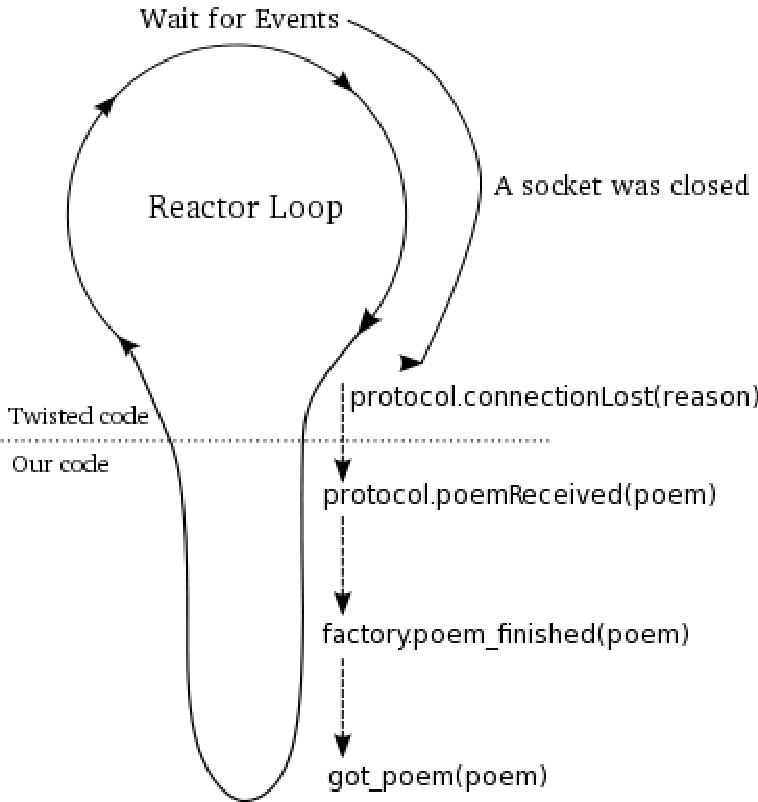
\includegraphics[height=0.3\textheight]{images/reactor-poem-callback.pdf}
    \caption{поэтические callback'и\label{fig:reactor-poem-callback}}
\end{center}
\end{figure}


%Figure 11 is worth contemplating. Up until now we have depicted callback chains that terminate with a single call to “our code”. But when you are programming with Twisted, or any single-threaded reactive system, these callback chains might well include bits of our code making callbacks to other bits of our code. In other words, the reactive style of programming doesn’t stop when it reaches code we write ourselves. In a reactor-based system, it’s callbacks all the way down.

Рисунок \ref{fig:reactor-poem-callback} стоит созерцания. 
До сих пор мы изображали цепочки callback'ов, которые 
завершались одним вызовом "нашего кода". Но когда вы 
программируете с Twisted, или любой другой однопоточной  
реактивной системой, эти цепочки callback'ов могут включать 
небольшие куски вашего кода, которые делают вызовы других 
небольших кусков кода. Другими словами, реактивный 
стиль программирования не прекращается, когда он дошел до 
кода, который мы сами написали. В системе, основанной на 
реакторе, все callback'и последовательно 
вызываются.

%Keep that fact in mind when choosing Twisted for a project. When you make this decision:
Запомните этот факт при выборе Twisted для вашего проекта. 
Когда вы сделаете решение:

%    I’m going to use Twisted!

\hspace{10mm}
Я собираюсь использовать Twisted!

%You are also making this decision:
Вы также делаете решение:

%    I’m going to structure my program as a series of asynchronous callback chain invocations powered by a reactor loop!

\hspace{10mm}
Я собираюсь структурировать мою программу как серию 
асинхронной callback цепочки, вызовы элементов которой 
осуществляются из цикла реактора!


%Now maybe you won’t exclaim it out loud the way I do, but it is nevertheless the case. That’s how Twisted works.
Теперь может быть вы не будете восклицать это так громко как это написано, 
но это тем не менее это повод. Это то, как работает Twisted.


%It’s likely that most Python programs are synchronous and most Python modules are synchronous too. If we were writing a synchronous program and suddenly realized it needed some poetry, we might use the synchronous version of our get_poetry function by adding a few lines of code to our script like these:

Вероятно, что большинство Python программ - синхронные, и 
большинство Python модулей - тоже синхронные. Если бы мы 
писали синхронную программу и внезапно поняли, что нам 
нужно немного поэзии, мы могли бы использовать 
синхронную версию нашей функции get\_poetry, добавляя 
несколько строк кода к нашему скрипту пободно следующим:


\begin{scriptsize}\begin{verbatim}
...
import poetrylib # I just made this module name up
poem = poetrylib.get_poetry(host, port)
...
\end{verbatim}\end{scriptsize}

%And continue on our way. If, later on, we decided we didn’t really want that poem after all then we’d just snip out those lines and no one would be the wiser. But if we were writing a synchronous program and then decided to use the Twisted version of get_poetry, we would need to re-architect our program in the asynchronous style using callbacks. We would probably have to make significant changes to the code. Now, I’m not saying it would necessarily be a mistake to rewrite the program. It might very well make sense to do so given our requirements. But it won’t be as simple as adding an import line and an extra function call. Simply put, synchronous and asynchronous code do not mix.

Давайте продолжим наш путь. Если позже мы решили бы, 
что, в конце концов, мы не хотим поэму, мы бы просто убрали бы 
эти строки. Но, если бы мы 
писали синхронную программу и затем решили бы использовать 
Twisted версию get\_poetry, нам нужно было бы перестроить 
нашу программу в асинхронном стиле, используя callback'и. 
Нам, вероятно,нужно было бы сделать значительные изменения в коде. 
При этом не утверждается, что переписать программу - это ошибка. 
Может быть очень хорошо так и сделать. Но это не будет так просто, как 
добавить строку с import и дополнительным вызовом функции. 
Или проще: синхронный и асинхронный код не смешиваются.  

%If you are new to Twisted and asynchronous programming, I might recommend writing a few Twisted programs from scratch before you attempt to port an existing codebase. That way you will get a feel for using Twisted without the extra complexity of trying to think in both modes at once as you port from one to the other.

Если вы новичок в Twisted и в асинхронном программирования, то 
рекомендуется написать несколько Twisted программ с нуля до того, как 
вы попробуете портировать существующий код. Этим способом вы получите 
ощущение от использования Twisted без дополнительной сложности, 
чем пытаясь подумать в обоих режимах, когда вы портируете с одного на 
другой.

%If, however, your program is already asynchronous then using Twisted might be much easier. Twisted integrates relatively smoothly with pyGTK and pyQT, the Python APIs for two reactor-based GUI toolkits.

Если, однако, ваша программа уже асинхронная, то 
использование Twisted может быть намного проще. Twisted 
интегрирован относительно хорошо с 
\href{http://pygtk.org/}{pyGTK} и
\href{http://wiki.python.org/moin/PyQt}{pyQT}, python API 
для двух основанных на реакторе GUI библиотек.

%When Things Go Wrong
\subsection{Когда дела плохи}

%In client 3.0 we no longer detect a failure to connect to a poetry server, an omission which causes even more problems than it did in client 1.0. If we tell client 3.0 to download a poem from a non-existent server then instead of crashing it just waits there forever. The clientConnectionFailed callback still gets called, but the default implementation in the ClientFactory base class doesn’t do anything at all. So the got_poem callback is never called, the reactor is never stopped, and we’ve got another do-nothing program like the ones we made in Part 2.

В клиенте 3.0 мы больше не будем определять 
обработчик ошибки соединения с поэтическим сервером, 
упущение которой вызывает гораздо больше проблем, чем в клиенте 1.0. 
Если мы скажем клиенту 3.0 скачать поэму из несуществуюшего 
сервера, то вместо того, чтобы завершиться с ошибкой, он будет крутиться в вечном цикле. 
Метод clientConnectionFailed все еще вызовется, но 
реализация по умолчанию базового класса 
\href{http://twistedmatrix.com/trac/browser/tags/releases/twisted-8.2.0/twisted/internet/protocol.py#L103}{ClientFactory} 
ничего не 
делает. Поэтому мы получим никогда не вызывающийся callback got\_poem,
reactor никогда не остановится и мы получим еще одну ничего 
не делающую программу, подобно той, что мы делали в главе 2.


%Clearly we need to handle this error, but where? The information about the failure to connect is delivered to the factory object via clientConnectionFailed so we’ll have to start there. But this factory is supposed to be re-usable, and the proper way to handle an error will depend on the context in which the factory is being used. In some applications, missing poetry might be a disaster (No poetry?? Might as well just crash). In others, maybe we just keep on going and try to get another poem from somewhere else.

Ясно, что нам нужно управлять этой ошибкой, но где? 
Информация об ошибке соединения доставляется объекту 
Factory через clientConnectionFailed, поэтому мы должны 
начать здесь. Но предполагается, что Factory переиспользуема, и 
правильный путь - управлять ошибкой взависимости от контекста, 
в котором Factory используется. В некоторых приложениях, 
отсутствие поэзии может быть бедствием (Нет поэзии? Может быть равносильно 
критической ситуации). В других - можно продолжать работать и попробовать 
скачать другую поэму из другого места.   

%In other words, the users of get_poetry need to know when things go wrong, not just when they go right. In a synchronous program, get_poetry would raise an Exception and the calling code could handle it with a try/except statement. But in a reactive program, error conditions have to be delivered asynchronously, too. After all, we won’t even find out the connection failed until after get_poetry returns. Here’s one possibility:

Другими словами, пользователям get\_poetry нужно 
знать, когда дела плохи, и не только, когда все хорошо. 
В синхронной программе, get\_poetry могла бы генерировать 
исключение и вызывающий код мог бы его обрабатывать с 
помощью конструкции try/except. Но в реактивной программе, 
условие ошибки должно доставляться асинхронно. После этого, 
мы даже не обнаружим ошибку в соединении до тех пор, пока 
не возвратится get\_poetry. Далее одна из возможностей:

\begin{scriptsize}\begin{verbatim}
def get_poetry(host, port, callback):
    """
    Download a poem from the given host and port and invoke

      callback(poem)

    when the poem is complete. If there is a failure, invoke:

      callback(None)

    instead.
    """
\end{verbatim}\end{scriptsize}

%By testing the callback argument (i.e., if poem is None) the client can determine whether we actually got a poem or not. This would suffice for our client to avoid running forever, but that approach still has some problems. First of all, using None to indicate failure is somewhat ad-hoc. Some asynchronous APIs might want to use None as a default return value instead of an error condition. Second, a None value carries a very limited amount of information. It can’t tell us what went wrong, or include a traceback object we can use in debugging. Ok, second try:

Проверяя аргумент callback'а (например, если poem is None), 
клиент может определить действительно ли мы имеем поэму или нет. 
Это могло бы быть достаточным для нашего клиента для того, чтобы 
избежать вечного запуска, но это метод все еще имеет 
некоторые проблемы. Прежде всего, использовать None для индикации 
ошибки - это нечно специальное. Некоторые асинхронные API могут 
захотеть использовать None в качестве возвращаемого 
значения по умолчанию вместо условия ошибки. Во-вторых, значение None 
приносит очень мало информации. Оно не может сказать нам, что пошло 
не так, или включить объект traceback, который мы могли бы 
использовать для отладки. Хорошо, вторая попытка:

\begin{scriptsize}\begin{verbatim}
def get_poetry(host, port, callback):
    """
    Download a poem from the given host and port and invoke

      callback(poem)

    when the poem is complete. If there is a failure, invoke:

      callback(err)

    instead, where err is an Exception instance.
    """
\end{verbatim}\end{scriptsize}

%Using an Exception is closer to what we are used to with synchronous programming. Now we can look at the exception to get more information about what went wrong and None is free for use as a regular value. Normally, though, when we encounter an exception in Python we also get a traceback we can analyze or print to a log for debugging at some later date. Tracebacks are extremely useful so we shouldn’t give them up just because we are using asynchronous programming.

Использование Exception ближе к тому, что 
мы используем в синхронном программировании. Теперь 
мы посмотрим на исключение для получения большей информации 
о том, что плохого произошло и освободим None 
для использования в качестве регулярного значения. Хотя это нормально, 
что когда мы сталкиваемся с исключением в Python'е, 
мы также получаем traceback, мы можем анализировать или печатать 
лог для отладки немногим позже. Traceback'и особенно полезны, поэтому 
мы должны их передавать наверх при использовании 
асинхронного программирования.

%Keep in mind we don’t want a traceback object for the point where our callback is invoked, that’s not where the problem happened. What we really want is both the Exception instance and the traceback from the point where that exception was raised (assuming it was raised and not simply created).

Запомните, что мы не хотим получить объект traceback в месте 
вызова нашего callback'а, так как это не то место, где произошла 
проблема. Что мы действительно хотим так это экземпляр Exception и 
traceback в месте, где произошло исключение (предполагая, что оно 
произошло, а не просто было создано).


%Twisted includes an abstraction called a Failure that wraps up both an Exception and the traceback, if any, that went with it. The Failure docstring explains how to create one. By passing Failure objects to callbacks we can preserve the traceback information that’s so handy for debugging.

Twisted включает абстракцию, называемую 
\href{http://twistedmatrix.com/trac/browser/tags/releases/twisted-8.2.0/twisted/python/failure.py#L121}{Failure}, 
которая 
обертывает Exception и traceback. 
\href{http://twistedmatrix.com/trac/browser/tags/releases/twisted-8.2.0/twisted/python/failure.py#L141}{Строка с документацией} 
Failure объясняет как создать этот объект. Передавая объекты Failure в 
callback'и, мы сохраняем информацию о traceback'е, что очень 
удобно при отладке.

%There is some example code that uses Failure objects in twisted-failure/failure-examples.py. It shows how Failures can preserve the traceback information from a raised exception, even outside the context of an except block. We won’t dwell too much on making Failure instances. In Part 7 we’ll see that Twisted generally ends up making them for us.

В 
\href{http://github.com/jdavisp3/twisted-intro/blob/master/twisted-failure/failure-examples.py}{twisted-failure/failure-examples.py} 
находится пример кода, который использует объекты типа Failure. 
В этом примере показано как Failures может сохранять 
информацию о traceback'е из возникшего исключения, даже вне 
контекста блока except. Мы не будем подробно останавливаться на 
создании экземпляров типа Failure. В главе 7 мы посмотрим на то, 
как Twisted в целом создает их для нас.


%Alright, third try:
Хорошо, третья попытка:

\begin{scriptsize}\begin{verbatim}
def get_poetry(host, port, callback):
    """
    Download a poem from the given host and port and invoke

      callback(poem)

    when the poem is complete. If there is a failure, invoke:

      callback(err)

    instead, where err is a twisted.python.failure.Failure instance.
    """
\end{verbatim}\end{scriptsize}


%With this version we get both an Exception and possibly a traceback record when things go wrong. Nice.
В этой версии мы получили оба - Exception и traceback на 
момент проблемы. Прекрасно.


%We’re almost there, but we’ve got one more problem. Using the same callback for both normal results and failures is kind of odd. In general, we need to do quite different things on failure than on success. In a synchronous Python program we generally handle success and failure with two different code paths in a try/except statement like this:
Мы практически все сделали, но у нас есть еще одна проблема. 
Использовать один и тот же callback для нормального и проблемного  
результатов - это странно. Обычно, нам нужно сделать нечто отличное
 в случае проблемы, чем в успешном исходе. 
В синхронной Python программе мы обычно управляем успешными и 
проблемными исходами в двух различных ветках оператора try/exception 
примерно так:

\begin{scriptsize}\begin{verbatim}
try:
    attempt_to_do_something_with_poetry()
except RhymeSchemeViolation:
    # the code path when things go wrong
else:
    # the code path when things go so, so right baby
\end{verbatim}\end{scriptsize}


%If we want to preserve this style of error-handling, then we need to use a separate code path for failures. In asynchronous programming a separate code path means a separate callback:
Если мы хотим сохранить такой стиль управления ошибками, то нам 
нужно использовать отдельную ветку в случае возникновления проблем. 
В асинхронном программировании отдельная ветка означает отдельный 
callback: 

\begin{scriptsize}\begin{verbatim}
def get_poetry(host, port, callback, errback):
    """
    Download a poem from the given host and port and invoke

      callback(poem)

    when the poem is complete. If there is a failure, invoke:

      errback(err)

    instead, where err is a twisted.python.failure.Failure instance.
    """
\end{verbatim}\end{scriptsize}

\subsection{Клиент 3.1}

%Now that we have an API with reasonable error-handling semantics we can implement it. Client 3.1 is located in twisted-client-3/get-poetry-1.py. The changes are pretty straightforward. The PoetryClientFactory gets both a callback and an errback, and now it implements clientConnectionFailed:

Теперь у нас есть API с разумной семантикой управления 
ошибками, которую мы можем реализовать. Клиент 3.1 расположен в
\href{http://github.com/jdavisp3/twisted-intro/blob/master/twisted-client-3/get-poetry-1.py}{twisted-client-3/get-poetry-1.py}. 
Изменения достаточно простые. 
\href{http://github.com/jdavisp3/twisted-intro/blob/master/twisted-client-3/get-poetry-1.py#L66}{PoetryClientFactory} 
получает оба: callback и errback, и теперь в классе реализован 
метод clientConnectionFailed:

\begin{scriptsize}\begin{verbatim}
class PoetryClientFactory(ClientFactory):

    protocol = PoetryProtocol

    def __init__(self, callback, errback):
        self.callback = callback
        self.errback = errback

    def poem_finished(self, poem):
        self.callback(poem)

    def clientConnectionFailed(self, connector, reason):
        self.errback(reason)
\end{verbatim}\end{scriptsize}


%Since clientConnectionFailed already receives a Failure object (the reason argument) that explains why the connection failed, we just pass that along to the errback.
Поскольку 
\href{http://twistedmatrix.com/trac/browser/tags/releases/twisted-8.2.0/twisted/internet/protocol.py#L118}{clientConnectionFailed} 
получает объект типа Failure (в аргументе reason), 
который объясняет почему не произошло соединение, нам нужно 
только передать этот аргумент в errback. 


%The other changes are all of a piece so I won’t bother posting them here. You can test client 3.1 by using a port with no server like this:
Другие изменения мы не будем обсуждать, их можно посмотреть в коде. 
Вы можете запустить клиент 3.1, используя порт без сервера 
следующим образом:

\begin{scriptsize}\begin{verbatim}
python twisted-client-3/get-poetry-1.py 10004
\end{verbatim}\end{scriptsize}


%And you’ll get some output like this:
И вы получите следующий вывод:

\begin{scriptsize}\begin{verbatim}
Poem failed: [Failure instance: Traceback (failure with no frames): : Connection was refused by other side: 111: Connection refused.
]
\end{verbatim}\end{scriptsize}


%That’s from the print statement in our poem_failed errback. In this case, Twisted has simply passed us an Exception rather than raising it, so we don’t get a traceback here. But a traceback isn’t really needed since this isn’t a bug, it’s just Twisted informing us, correctly, that we can’t connect to that address.
Это напечатано оператором print в нашем poem\_failed 
errback'е. В этом случае Twisted просто передает 
исключение вместо его порождения, поэтому в данном 
случае мы не получаем traceback. Но traceback реально не 
нужен, поскольку это не ошибка, и Twisted корректно информирует 
нас, что мы не можем установить соединение по адресу.


\subsection{Резюме}

%Here’s what we’ve learned in Part 6:
Вот что мы изучили в этой главе:

\begin{itemize}
%    * The APIs we write for Twisted programs will have to be asynchronous.
\item API, которые мы пишем для Twisted программ, должны быть асинхронными.
%    * We can’t mix synchronous code with asynchronous code.
\item Мы не можем смешивать синхронный и асинхронный код.
%    * Thus, we have to use callbacks in our own code, just like Twisted does.
\item Таким образом, мы должны использовать callback'и в нашем коде, подобно 
тому как это делает Twisted.
%    * And we have to handle errors with callbacks, too.
\item Мы должны управлять ошибками в callback'ах.
\end{itemize}


%Does that mean every API we write with Twisted has to include two extra arguments, a callback and an errback? That doesn’t sound so nice. Fortunately, Twisted has an abstraction we can use to eliminate both those arguments and pick up a few extra features in the bargain. We’ll learn about it in Part 7.
Значит ли, что каждый API, который мы написали с помощью 
Twisted должен включать два дополнительных аргумента, 
callback и errback? Это звучит не так приятно. 
К счастью, Twisted имеет абстракцию, которую мы можем 
использовать для того, чтобы исключить оба этих аргумента 
и преобрести несколько дополнительных свойств. 
Мы узучим это в следующей главе.

\subsection{Упражнения}

\begin{enumerate}
%1. Update client 3.1 to timeout if the poem isn’t received after a given period of time. Invoke the errback with a custom exception in that case. Don’t forget to close the connection when you do.
\item Обновите клиент 3.1 и установите timeout, который 
активизируется, если поэма не получена после заданного 
интервала времени. В этом случае вызывайте errback с пользовательским исключением. 
Не забудьте закрыть соединение. 
%   2. Study the trap method on Failure objects. Compare it to the except clause in the try/except statement.
\item Изучите метод trap объектов Failure. Сравните его с условием except в операторе try/except.
%   3. Use print statements to verify that clientConnectionFailed is called after get_poetry returns.
\item Используйте оператор print для того, чтобы убедиться, что clientConnectionFailed 
вызывается после выхода из get\_poetry.
\end{enumerate}

